%% =====================================================================
%% 多代理人立場交換辯論機制應用於投資決策（初稿）
%% 2026-10-06 新版研究設計修訂稿；bibliography 已嵌入。原介面圖片存在時沿用，否則呈現文字說明。
%% 章節依系上專題報告格式：摘要、引言、文獻探討、研究方法、
%% 系統設計與實作、結果與討論、結論與建議、參考文獻（APA）
%% =====================================================================

\documentclass[12pt,a4paper]{article}

%% ---------- 套件 ----------
\usepackage[T1]{fontenc}
\usepackage{newtxtext}
\usepackage{amsmath}
\usepackage[left=2.5cm,right=2.5cm,top=2.5cm,bottom=2.5cm]{geometry}
\usepackage{CJKutf8}
\usepackage{graphicx,array,tabularx,booktabs,float}
\usepackage{setspace,enumitem,footmisc}
\usepackage[explicit]{titlesec}
\usepackage{caption}
\usepackage{natbib}
\usepackage{tikz}
\usetikzlibrary{positioning,arrows.meta,calc}
\usepackage[bookmarks=false,hidelinks]{hyperref}

%% ---------- 行距與段落 ----------
\setstretch{1.5}
\setlength{\parindent}{2em}
\setlength{\parskip}{0pt}
\setlist{itemsep=2pt,topsep=4pt,leftmargin=2.5em}
\renewcommand{\arraystretch}{1.3}
\setlength{\footnotesep}{8pt}
\emergencystretch=2em

%% ---------- 中文數字編號 ----------
\newcommand{\chnum}[1]{\ifcase#1\or 一\or 二\or 三\or 四\or 五\or 六\or 七\or 八\or 九\or 十\fi}
\renewcommand{\thesection}{\chnum{\value{section}}}
\renewcommand{\thesubsection}{（\chnum{\value{subsection}}）}

%% ---------- 標題 ----------
\titleformat{\section}{\fontsize{16}{24}\selectfont}{\thesection、}{0em}{#1}
\titleformat{\subsection}{\fontsize{14}{21}\selectfont}{\thesubsection}{0em}{#1}
\titleformat{\paragraph}[runin]{\fontsize{12}{18}\selectfont}{}{0em}{#1}
\titleformat{name=\section,numberless}{\fontsize{16}{24}\selectfont}{}{0em}{#1}
\titlespacing*{\section}{0pt}{18pt}{12pt}
\titlespacing*{\subsection}{0pt}{12pt}{6pt}
\titlespacing*{\paragraph}{2em}{6pt}{0.5em}

%% ---------- 圖表 ----------
\captionsetup{font={small,stretch=1.2},labelsep=quad,skip=6pt}
\captionsetup[table]{position=top}
\setlength{\heavyrulewidth}{0.8pt}
\setlength{\lightrulewidth}{0.4pt}
\pagestyle{plain}

\newcommand{\grp}[1]{\textsf{#1}}
\newcolumntype{Y}{>{\raggedright\arraybackslash}X}

\begin{document}
\begin{CJK}{UTF8}{bkai}

\renewcommand{\refname}{參考文獻}
\renewcommand{\tablename}{表}
\renewcommand{\figurename}{圖}

%% =====================================================================
%% 封面
%% =====================================================================
\begin{titlepage}
\centering
\setstretch{1.6}
\vspace*{2cm}
{\fontsize{18}{27}\selectfont 國立陽明交通大學管理科學系\par}
\vspace{0.3cm}
{\fontsize{16}{24}\selectfont 專題研究報告\par}
\vspace{3.5cm}
{\fontsize{20}{32}\selectfont 多代理人立場交換辯論機制\\ 應用於投資決策\par}
\vspace{0.3cm}
{\fontsize{12}{18}\selectfont 模型異質性與領域專業化之延伸\par}
\vspace{0.5cm}
{\fontsize{14}{21}\selectfont Multi-Agent Role-Switching Debate\\ for Investment Decision-Making\par}
\vfill
{\fontsize{14}{24}\selectfont
\begin{tabular}{r@{\hspace{1.5em}}l}
學\hspace{2em}生： & 黃岳振 \\
指導教授： & 林斯寅\ 教授 \\
\end{tabular}\par}
\vspace{2.5cm}
{\fontsize{14}{21}\selectfont 中華民國一一五年十月\par}
\vspace{1.5cm}
\end{titlepage}

%% =====================================================================
%% 摘要
%% =====================================================================
\pagenumbering{roman}
\begin{center}
{\fontsize{16}{24}\selectfont 摘\quad 要\par}
\end{center}
\vspace{0.3cm}


投資決策需要整合技術面、基本面、新聞情緒與總體經濟資訊，不同證據可能互相衝突。多代理人辯論透過多空觀點與裁決程序檢查論證，但角色差異不必然形成有效的推理差異。本研究以自我反駁式立場交換為核心，探討三個層次：立場交換相對固定立場辯論的增量價值、模型組成是否改變此效果，以及領域專業化的決策分工是否改善績效與成本效益。研究採九檔美國大型股於2021至2025年的180個季度案例，整合四類金融資訊，並透過時間邊界、不可變資料快照、證據識別碼與稽核紀錄維持比較的一致性。主要評估指標為60個交易日方向準確率與年化Sharpe比率，輔以報酬、回撤、決策分歧及推論資源指標。

\vspace{0.6cm}
\noindent 關鍵詞：大型語言模型、多代理人辯論、立場交換、模型異質性、領域專業化、投資決策
\clearpage
\begin{center}{\fontsize{16}{24}\selectfont Abstract\par}\end{center}
\noindent Investment decisions require the integration of technical, fundamental, news-sentiment and macroeconomic evidence, which may conflict. Multi-agent debate uses opposing views and adjudication to examine arguments, yet role differences do not necessarily produce useful reasoning diversity. This study retains self-rebuttal role-switching as its core and investigates three levels: its incremental value over fixed-role debate, whether model composition changes this effect, and whether domain-specialized decision-making improves performance and cost effectiveness. The study uses 180 quarterly cases of nine U.S. stocks in 2021--2025, integrating four financial information domains under point-in-time data boundaries, immutable snapshots, evidence identifiers and audit trails. The primary evaluation metrics are 60-trading-day directional accuracy and annualized Sharpe ratio, supplemented by return, drawdown, disagreement and inference-resource measures.

\vspace{0.6cm}
\noindent Keywords: large language models, multi-agent debate, role switching, model heterogeneity, domain specialization, investment decisions
\clearpage
\tableofcontents
\clearpage
\pagenumbering{arabic}

\section{引言}

\subsection{研究背景}

\subsubsection{金融資訊整合與大型語言模型}
投資決策同時涉及技術面、基本面、新聞情緒與總體經濟資訊；這些證據的時間尺度、資料形式與方向可能不同。大型語言模型可輔助閱讀財報、新聞與市場資料，並已用於金融語言處理與投資分析 \citep{lopezlira2023chatgpt,araci2019finbert,liu2023fingpt}。然而，資訊整合與未來報酬預測是不同任務，流暢的敘事不保證有用的預測訊號。

\subsubsection{Multi-Agent Debate 與 Role-Switching}
多代理人辯論讓不同角色提出、批評與修正論點 \citep{du2023debate,liang2023divergent}，金融代理人系統也採用分析與交易角色分工 \citep{xiao2024tradingagents,zhang2024stockagent}。辯論的效果受模型、互動與裁決程序影響，並不必然優於單一模型或獨立投票 \citep{smit2023mad,zhang2025stop}，因此工作流的配置本身也是研究對象。

本研究以固定立場辯論C與自我反駁式立場交換D為核心比較。D第二輪只讀自己的第一輪論述，引用並反駁原主張，第三輪回到原始立場整合反證。此機制檢驗重新檢查既有證據的增量價值，並延伸至模型組成與決策層領域分工。

\subsection{研究動機}

\subsubsection{自我反駁機制的增量價值}
多代理人辯論的效果仍有爭議：部分研究顯示辯論可提升推理正確性 \citep{du2023debate}，但也有研究發現辯論不一定優於多次取樣投票，且效果常被高估 \citep{smit2023mad,zhang2025stop}。辯論的已知問題之一是代理人「固守立場」，只強化自己的論點而不回應反面證據；立場交換被提出以緩解此問題 \citep{liu2025roleswitch,chowdhury2026proclaim}。這些研究提供角色交換的機制動機，但其任務與未來金融報酬預測不同；本研究因而直接比較相同資料與名目決策呼叫次數下的C/D流程。此外，金融回測特別容易失真：模型可能記得回測期間的後續走勢 \citep{glasserman2023lookahead,kong2026bias}，辯論組也通常比單次判斷多用數倍的模型呼叫。因此，本專題希望在控制這些偏誤的條件下，檢驗立場交換在投資情境是否真的有用。
\subsubsection{模型同質性與推理差異}

Bull 與 Bear 雖有相反角色提示，使用相同基礎模型時仍可能共享知識邊界、推理偏好與錯誤。角色差異不保證有效推理差異；異質模型是否提供互補性仍需檢驗 \citep{zhang2025stop}。不同模型的能力、訓練資料及輸出風格也可能不同，因此模型替換帶來的績效差不能直接歸因於異質性。

\subsubsection{Generalist 資訊集中與領域分工}

既有四個研究代理人提供資料整理分工，決策推理仍集中於共同 Bull/Bear。技術、基本、新聞情緒與總經證據的時間尺度及訊號型態不同，合併後可能壓縮特定領域反證或增加 context 負擔。此為研究假說，不是已由舊負面結果證實的原因。RQ3 將分工延伸至領域內多空論證，再由上層整合，評估收益、衝突與資源負擔。

\subsection{研究目的}

\subsubsection{立場交換機制}
檢驗自我反駁式立場交換相對固定立場辯論的增量價值，維持原核心問題。

\subsubsection{模型異質性}
檢驗同一辯論內的模型組成是否改變 D 相對 C 的效果，區分角色差異與模型差異。

\subsubsection{領域專業化}
檢驗領域內辯論及上層整合相對 Generalist 的績效與成本，評估任務分解的價值。

\subsection{Research Questions}

\subsubsection{RQ1 原始機制}
\begin{quote}在相同案例資料與相同名目決策呼叫次數下，自我反駁式立場交換辯論（D）的 60 日方向準確率與年化 Sharpe 是否高於固定立場辯論（C）？\end{quote}

\subsubsection{RQ2 Model Heterogeneity}
\begin{quote}當看多與看空代理人由不同基礎模型擔任時，自我反駁式立場交換辯論（D）相對固定立場辯論（C）的投資決策效果是否改變？\end{quote}

\subsubsection{RQ3 Domain-Specialized Debate}
\begin{quote}相較於將四類金融資訊整合後交由共同多空代理人辯論，若改由技術面、基本面、情緒面與總經面代理人分別在各自資訊領域進行多空辯論，再由上層整合機制形成最終投資決策，是否能改善方向準確率與風險調整後績效？\end{quote}
三題構成機制、模型組成與任務分工的連續研究：RQ1檢驗核心機制，RQ2檢驗模型層差異，RQ3檢驗決策架構的領域分工。

\subsection{研究範圍}

\subsubsection{樣本與資料時間邊界}
本專題定位為投資決策輔助之研究與系統原型，不是自動交易系統，範圍如表~\ref{tab:scope}。

\begin{table}[H]
\centering\small
\caption{研究範圍}
\label{tab:scope}
\begin{tabularx}{\textwidth}{@{}l Y@{}}
\toprule
面向 & 範圍說明 \\
\midrule
標的與期間 & 九檔美國大型股，2021 至 2025 年每季一個分析日，共 180 個案例 \\
資料 & 技術面、基本面、情緒面（新聞標題）與總經面，僅使用分析日前已公開之資料 \\
決策輸出 & 買進、持有或賣出，以及預期報酬、信心度、理由、引用證據與風險 \\
評估 & 60 個交易日之方向準確率與 Sharpe 比率；30 與 90 日為穩健性檢查 \\
\bottomrule
\end{tabularx}
\end{table}
\subsubsection{預測期間與決策層}

維持九股、20 季末、180 個 stock $\times$ date cases、60 trading days。C/D 候選裁決沿用 Buy/Sell，Gatekeeper 可降為 Hold 或不交易；A/B 允許 Hold，僅作補充對照。主要分析沿用候選決策層，守門後實際風險處理另列敏感性。原月度／20 日比較移至未來展望，不任意替換正式樣本。

\section{文獻探討}

\subsection{Multi-Agent Debate}

\subsubsection{辯論與自我一致性的公平對照}
\citet{du2023debate} 讓多個模型實例進行多輪辯論後收斂答案，改善推理與事實正確性；\citet{liang2023divergent} 指出模型自我反思容易固守既有答案，並以辯論鼓勵發散思考。另一方面，\citet{smit2023mad} 比較多種辯論策略，顯示多代理人辯論不一定穩定優於自我一致性等其他方法，且對設定敏感；\citet{zhang2025stop} 主張目前的評估常高估辯論，呼籲重新思考評估方式並採用異質模型。自我一致性 \citep{wang2023selfconsistency} 以多次取樣投票提升穩定性，是比較辯論效果時必要的對照組，本研究的獨立投票組即據此設計。由此，本研究把重點放在可追蹤的流程與公平比較（呼叫次數對齊），而不是預設辯論一定比較準。
\subsection{Role-Switching / Self-Rebuttal}

\subsubsection{機制假說與失效條件}
\citet{liu2025roleswitch} 提出不確定性感知的角色交換辯論：兩個辯論者先給出初始答案並互相詰問，再於辯論中途交換角色論證相反立場，然後各自回報信心與不確定性，最後由另一個裁判模型裁決；在 OpenBookQA 上，其消融實驗顯示角色交換與不確定性回報兩個階段均有貢獻。\citet{chowdhury2026proclaim} 的 PROCLAIM 以法庭角色（原告、辯護、法官）與漸進式檢索進行主張查核，並以角色交換作為一致性診斷；其消融結果顯示角色交換帶來約 4.2 個百分點的準確率提升，但整體 token 用量約為標準多代理人辯論的 11 倍。\citet{chen2026mpt} 的多人格思考以相反的人格與中立觀點反覆對話，使偏誤外顯並被修正。這些研究支持「從相反立場重新思考」的想法，但皆非投資決策，且第二項的效益是伴隨成本增加而來，凸顯呼叫預算對齊的必要。本研究因此採用看多、看空與裁決者的三角架構，並讓獨立投票與兩辯論組之決策呼叫次數對齊（單次判斷為基準）。\paragraph{機制動機與可能失效的條件。}
\citet{lord1984opposite} 的人類社會判斷實驗指出，考慮與既有信念相反的可能性可減少特定判斷偏誤。本研究據此提出機制假說：要求代理人引用並反駁自己的論點，可能暴露先前忽略的反證，改善裁決對證據的權衡。此推論從人類判斷延伸至 LLM 金融預測，尚須實證檢驗；論述更完整不必然代表未來報酬預測更準確。\citet{huang2024selfcorrect} 發現，缺乏外部回饋的內生自我修正，在其推理基準上可能無效甚至降低表現；若模型共享相同錯誤、輸入資訊缺乏預測訊號，或市場噪音主導結果，自我反駁也可能只改變敘事而無績效增益。


\subsection{Model Heterogeneity in Multi-Agent Systems}

\subsubsection{異質性、能力組成與模型偏向}

\citet{zhang2025stop} 對多代理人辯論評估與模型異質性提出檢驗，提供不同底層模型共同推理的研究動機。其基準結果不能直接外推到金融未來報酬或本研究自我反駁規則。RQ2 將同一辯論內 A/B 共存與整套系統換成 B 區分；後者仍是 homogeneous setting。模型能力、偏向、Judge 親和與錯誤相關性須分別診斷。

\citet{wang2024moa} 的Mixture-of-Agents將多個模型的輸出逐層整合，並比較相同模型重複生成與多模型提案。該研究也區分提案與整合角色，說明模型在不同工作流位置的適用性可能不同。本研究據此將模型組成視為實驗因素，同時固定裁決者；其一般語言任務結果不等於異質金融辯論有效，也不能排除模型能力差距。

\subsection{Financial LLM and Investment Agents}

\subsubsection{金融語言與代理人工作流}
\citet{lopezlira2023chatgpt} 在其樣本與設定中發現，LLM 對金融新聞標題的判讀含有與後續報酬相關的訊息；FinBERT \citep{araci2019finbert} 與 FinGPT \citep{liu2023fingpt} 提供金融語言處理方法，FNSPID \citep{dong2024fnspid} 則提供具時間戳記的新聞資料。這些工作說明資訊整理的可能用途，但不能直接推得任何辯論流程有增量價值。

TradingAgents \citep{xiao2024tradingagents} 與 StockAgent \citep{zhang2024stockagent} 將 LLM 分工與交易決策置於回測或模擬環境；其研究對象包含整套代理人系統，與本研究控制案例輸入後比較 \grp{D}、\grp{C} 的估計量不同。\citet{glasserman2023lookahead} 的前視風險分析，以及 \citet{huang2024selfcorrect} 對無外部回饋自我修正的審慎結果，均提醒：流暢推理與模擬績效不能單獨證明可用的未來預測訊號。本研究的缺口因而限定為：在名目呼叫次數對齊、資料時間邊界可稽核的設定下，重新檢查既有證據的自我反駁流程是否改善方向與風險調整績效，而非僅將既有辯論方法搬至金融領域。
\subsection{Domain Specialization / Task Decomposition}

\subsubsection{摘要分工與決策分工的區分}
TradingAgents與StockAgent提供金融代理人工作流的脈絡 \citep{xiao2024tradingagents,zhang2024stockagent}。FinRobot將金融任務分解為專業代理人與分層流程，提供金融問題分解與工具鏈設計的例子 \citep{yang2024finrobot}；它不直接提供本研究四領域多空辯論與Generalist架構的受控績效比較。

\citet{chen2023agentverse} 的AgentVerse區分專家配置、協作決策、執行與評估，並討論水平與垂直協作結構。其工作說明代理人分工與溝通結構可以共同塑造決策程序。RQ3因而將專業化從資料整理層延伸至領域內推理與上層整合；四類領域的切分是本研究的設計選擇，而非既有研究證明的最優架構。

領域切分可能保留局部反證，也可能遺失跨領域脈絡、增加摘要壓縮與整合誤差。相較於僅以context長度解釋分工，本研究關注專業化是否應進入決策推理層，並以績效、證據使用及推論資源評估其交換關係。

\subsection{Judge / Aggregation / Validation}
\subsubsection{論證生成、上層整合與證據驗證}
Mixture-of-Agents區分提案生成與上層整合 \citep{wang2024moa}，提供不同角色承擔論證與綜合工作的架構參考。\citet{zheng2023judge} 指出LLM裁判可能出現位置、冗長與自我偏好等偏誤，因此裁決輸入的順序、長度及模型標籤需要控制。該研究評估的是回答品質，不能直接證明本研究投資Judge的預測效力。

本研究據此將argument generation、decision aggregation與evidence validation分成可稽核步驟。Judge或Final Aggregator綜合論點形成方向，Gatekeeper則檢查證據存在性、資料覆蓋與風險條件。後者是本系統的驗證設計，不以一般LLM裁判文獻作為其能改善投資績效的證明。

\subsection{Look-Ahead Bias and Financial Evaluation}

\subsubsection{資料時間邊界與模型訓練記憶}
\citet{glasserman2023lookahead} 指出以 GPT 產生之情緒訊號預測報酬時，模型可能透過對公司的既有知識引入前視偏差，並嘗試以匿名化緩解；\citet{kong2026bias} 歸納金融 LLM 常見的五種偏誤（前視、存活、敘事、目標與成本偏誤），並指出多數研究未明確處理。本研究因而在資料端嚴格排除分析日以後的資訊，以舊協議的無資料回想與匿名辨識探針作前導風險診斷（舊協議前導診斷小節），並在回測中扣除交易成本。探針並非新版主樣本的完整汙染檢驗。
\subsection{Literature Synthesis / Research Gap}

\subsubsection{機制、模型與任務的連續問題}

本研究承接辯論、自我一致性、角色交換、金融語言處理與前視偏差文獻，從固定案例資料下自我反駁有無增量價值出發，再檢驗指定模型組成與領域分工是否改變決策。原文獻不足以證明同質性或資訊負荷已導致舊結果失效；新版三題提供可稽核比較，而不預設任何架構必然較佳。文獻中的問答正確性、事實查核與投資報酬預測端點不同，不能直接等同。原自我一致性、角色交換與負面結果來源皆保留。

\section{研究方法}

\subsection{研究架構}

\subsubsection{共同資料層與三個實驗分支}

既有 Coordinator、Data Snapshot 與四類 Research Agents 保留。共同資料層產生不含投資方向的鎖定研究資料與證據登錄。RQ1/RQ2 讀取同一 Neutral Report；RQ3 Generalist 仍讀整合報告，Domain 分支使用相同研究輸出的領域切片，不另抓新資料或以不同摘要模型重製輸入。概念架構如下。
\begin{figure}[H]\centering
\begin{tikzpicture}[node distance=6mm,box/.style={draw,align=center,font=\small,text width=125mm,inner sep=4pt},arr/.style={-{Stealth[length=2mm]}}]
\node[box] (data) {Data：同案例、filing date、historical vintage、timestamp};
\node[box,below=of data] (research) {Immutable Snapshot $\rightarrow$ Four Research Agents $\rightarrow$ Evidence Registry};
\node[box,below=of research] (branches) {RQ1：Homogeneous C/D，same Neutral Report\\RQ2：Heterogeneous C/D，AB/BA counterbalance\\RQ3：Generalist／四個 Domain Bull/Bear Debates};
\node[box,below=of branches] (judge) {RQ1/2 固定 Judge；RQ3 Final Judge / Aggregator};
\node[box,below=of judge] (gate) {既有 Gatekeeper：證據、資料覆蓋與風險驗證};
\node[box,below=of gate] (back) {Backtest $\rightarrow$ Accuracy / Sharpe / Cost / Diagnostics};
\draw[arr] (data)--(research);\draw[arr] (research)--(branches);\draw[arr] (branches)--(judge);\draw[arr] (judge)--(gate);\draw[arr] (gate)--(back);
\end{tikzpicture}
\caption{研究概念架構。三分支以共同資料、候選決策及評估口徑銜接。}\label{fig:flow}\end{figure}

\subsubsection{Judge 與 Gatekeeper}

Judge 綜合辯論、核對證據並形成投資方向。Final Aggregator 是 RQ3 整合四個 Domain Views 的上層裁決者，不再額外假設其後需要另一個決策 Judge。Gatekeeper 在投資方向形成後檢查引用、coverage、volatility、risk threshold、基準率歷史並必要時降級；它不承擔四領域投資觀點整合。

\subsection{資料收集}

\subsubsection{四類資料與時間控制}
樣本為九檔美國大型股（AAPL、\allowbreak NVDA、\allowbreak GOOGL、\allowbreak MSFT、\allowbreak AMZN、\allowbreak JPM、\allowbreak MCD、\allowbreak INTC、\allowbreak GE），分析日為 2021 至 2025 年共 20 個季末。每個案例只使用分析日前已公開之資料（表~\ref{tab:data}）：財報依申報日而非會計期末篩選，總經資料使用當時實際已發布之歷史版本，資料快照以內容雜湊識別，四組決策讀取同一份快照。

\begin{table}[H]
\centering\small
\caption{資料來源與處理方式}
\label{tab:data}
\begin{tabularx}{\textwidth}{@{}l l Y@{}}
\toprule
面向 & 來源 & 內容與處理 \\
\midrule
技術面 & 調整後日行情 & 近 20 日報酬、均線相對位置、年化波動度；僅用分析日前價格 \\
基本面 & SEC 財報 & 營收、淨利、營業現金流與去年同期比較；依申報日篩選 \\
情緒面 & 金融新聞標題（FNSPID、Alpha Vantage） & 分析日前 90 天全部標題，既有資料共83,093則，以 FinBERT 逐則評分後彙整 \\
總經面 & FRED／ALFRED & 失業率、利率、物價等，僅採分析日當時已發布之數值 \\
\bottomrule
\end{tabularx}
\end{table}

九檔選取以資料可取得性為主，並非依2021年成分股隨機抽樣。協議記錄排除新聞來源未涵蓋的ASTS，並以INTC替換有早期新聞缺口的LLY，因此樣本具有目的性選樣與存活偏誤風險。主要比較保留180案；既有排除37案分析僅視為新聞來源／覆蓋診斷，不使用其結果建立統一新聞密度門檻。

\subsubsection{資料品質與版本風險}
為確保快照僅反映分析日當時可得之資訊，本研究採取三項處理：其一，財報依申報日期而非會計期末篩選，並以相同會計科目、相同期間長度與前一年同期比較，避免混用不同期間；其二，年增率以前期絕對值為分母，使負數基期惡化時呈現負值，避免符號誤導；其三，快照以內容雜湊為識別碼，同一模型同一案例內的四組決策機制讀取同一份快照與鎖定報告。行情使用 yfinance 的 auto\_adjust=True；調整係數反映下載時可得之拆股與股利處理，並非各分析日保存的調整版本，仍有事後修訂風險。
新聞依發布 timestamp 與時區篩選，財報以 filing date 判定實際可得，macro 以分析日已發布的 historical vintage 建立；價格輸入只使用 cutoff 以前。每案記錄 data version、snapshot hash、evidence ID、code version、model version 與 audit trail。同案跨條件共用快照不能單獨證明資料內容正確，須驗證可用時間與來源。模型revision、新聞來源與調整行情下載版本均是影響精確重現的資料身分，須與快照及執行紀錄一併保存。

\subsection{研究設計選擇與理據}
\begin{table}[H]\centering\small
\caption{主要設計選擇及其研究功能}
\begin{tabularx}{\textwidth}{@{}l l Y@{}}\toprule
設計 & 設定 & 理據\\\midrule
辯論者 & Bull與Bear & 以兩個對立方向建立最小多空論證結構。\\
辯論輪次 & 三輪 & 初始論證、自我反駁與整合修正各占一輪；此為機制的操作化選擇，不宣稱最優輪數。\\
交換時點 & 第二輪 & 先形成可引用的原始主張，再要求反向檢查。\\
交換輪資訊 & 自身第一輪 & 將反駁對象限定自身主張，降低轉為模仿對手的可能。\\
第三輪 & 回原立場 & 整合反證與不確定性，觀察修正後論點。\\
裁決與驗證 & Judge後接Gatekeeper & 區分投資方向整合、證據有效性及風險控制。\\
主要比較 & C/D同名目呼叫數 & 控制一項推論資源差異，實際token與重試成本另報。\\
分析頻率 & 季度 & 配合財務資訊的季度更新節奏，維持原資料pipeline與20個決策時間點。\\
主要期間 & 60交易日 & 作為季度研究的操作性持有期間，30與90日檢查期間敏感性，不宣稱60日具有理論最適性。\\
資訊領域 & 技術、基本、情緒、總經 & 沿用既有四類證據，區分整理層與決策層的專業化。\\\bottomrule
\end{tabularx}\end{table}
模型輸出格式、引用匹配與重試屬實作參數；其功能在維持可執行與可稽核流程，與C/D、模型組成及任務架構等研究變因分開記錄。

\subsection{實驗設計}

\subsubsection{Common Experimental Setup}
各條件使用相同案例、資料快照、outcome與回測。研究代理人的模型與輸出、中立報告及證據登錄固定，避免更換辯論者時同時改變輸入資訊。C/D對齊三輪與Judge呼叫，模型設定、prompt hash、實際seed、token用量與重試均保存於稽核。

記憶只含分析日前已到期的同股票案例，禁止讀取該案例未來報酬或其他條件的測試結果。若採各條件自行累積的歷史記憶，後續輸入也受先前決策影響，因此比較量屬動態整套流程效果。實驗條件須控制記憶可見範圍，並記錄模型服務版本與截斷處理。

\subsubsection{Fixed-role Debate C}

C 的 Bull/Bear 三輪維持原始立場，每輪各一次呼叫，依原資訊可見規則批評與整合，再交固定 Judge，名目共七次。A 單次判斷、B 七次獨立投票僅供補充。四組流程如表~\ref{tab:arms}。
\paragraph{四組決策機制。} \grp{B}、\grp{C}、\grp{D} 三組之決策呼叫次數對齊（各 7 次），\grp{A} 為單次判斷之基準（表~\ref{tab:arms}）；此為名目呼叫數，D 的引用自身原文驗證可能另觸發重試；呼叫次數相同不代表實際重試次數、token 或運算量相同，辯論組因讀取歷史論述，輸入較長。每次決策輸出買進（做多）、持有（不進場）或賣出（放空），以及 60 個交易日之預期報酬、信心度、理由與引用證據。

\begin{table}[H]
\centering\small
\caption{四組決策機制}
\label{tab:arms}
\begin{tabularx}{\textwidth}{@{}c l c Y@{}}
\toprule
組別 & 名稱 & 呼叫次數 & 流程 \\
\midrule
\grp{A} & 單次判斷 & 1 & 讀取報告後直接決策 \\
\grp{B} & 獨立投票 & 7 & 同一提示獨立取樣七次，多數決 \\
\grp{C} & 固定立場辯論 & 7 & 看多與看空辯論三輪（每輪可見雙方論述），再由裁決者決策 \\
\grp{D} & 立場交換辯論 & 7 & 第二輪交換立場、只見自己第一輪並須反駁之，第三輪換回，再由裁決者決策 \\
\bottomrule
\end{tabularx}
\end{table}


\subsubsection{Role-Switching Debate D}
\paragraph{比較量。} 本專題估計整套 \grp{D} 對 \grp{C} 的複合流程效果差（composite-protocol estimand），包含立場交換、交換輪隔離對手、強制引用與相應驗證／重試。其比較同時包含多項處理，故不能歸因於單獨的立場交換。

\paragraph{立場交換辯論。} 表~\ref{tab:rounds} 為立場交換組之三輪流程。第二輪隔離對手論述是刻意設計：若同時看得到對手，代理人容易轉為回應對手，而非檢討自己的主張。辯論組之裁決者須逐項核對雙方引用之證據，並綜合雙方論點在買進與賣出之間擇一。

\begin{table}[H]
\centering\small
\caption{立場交換辯論之三輪流程}
\label{tab:rounds}
\begin{tabularx}{\textwidth}{@{}l Y Y@{}}
\toprule
輪次 & 內容 & 目的 \\
\midrule
第 1 輪 & 看多與看空代理人各自提出論點並引用證據 & 建立正反兩方初始立場 \\
第 2 輪 & 雙方交換立場，只能看到自己第一輪之論述，須引用並反駁自己的原主張 & 迫使代理人檢驗自身論點之弱點 \\
第 3 輪 & 雙方換回原立場，整合前兩輪之論點與反駁 & 產生整合後之論點與不確定性揭露 \\
裁決 & 讀取完整辯論與報告，逐項核對證據後擇一方向 & 避免以辯論聲量決定 \\
\bottomrule
\end{tabularx}
\end{table}


Model identity 在三輪固定：只有 stance 在第二輪反轉、第三輪回復。強制引用自己第一輪原文的驗證規則與重試屬處理的一部分，正式前保存 validator hash。現有原文核對採至少70\%字詞連續相同；這只檢查引用來源，不能證明反駁語意有效。

\subsubsection{RQ1 Design}
在相同案例資料與相同名目決策呼叫次數下，自我反駁式立場交換辯論（D）的 60 日方向準確率與年化 Sharpe 是否高於固定立場辯論（C）？

RQ1維持同質辯論者、同資料與七次名目決策呼叫，估計整套D相對C的方向準確率及Sharpe差。A/B僅作補充對照。股票代號與公司名稱在模型輸入中匿名化，並以版本鎖定與事前分析計畫維持執行規則的一致性。匿名化不排除數值、日期及產品線索造成的辨識；同批180案曾用於前導試跑與規則調整，因此其比較屬既有樣本的回溯分析，不視為未見樣本的獨立驗證。

\subsubsection{RQ2 Heterogeneous Model Design}

RQ2 主要操弄多空辯論者的模型組成；固定 case、snapshot、Neutral Report、Research Agents、三輪、Role-Switching rule、Judge、Gatekeeper、outcome與backtest。Homogeneous為A/A；Heterogeneous有兩個平衡配置：AB（原Bull=A、原Bear=B）與BA（原Bull=B、原Bear=A）。兩個配置均需有C與D，不讓A永遠是Bull。
\begin{table}[H]\centering\small
\caption{異質D的身份與立場，model identity不交換}
\begin{tabularx}{\textwidth}{@{}lYY@{}}\toprule
輪次 & AB配置 & BA配置\\\midrule
Round 1 & A Bull；B Bear & B Bull；A Bear\\
Round 2 & A Bear；B Bull & B Bear；A Bull\\
Round 3 & A Bull；B Bear & B Bull；A Bear\\\bottomrule\end{tabularx}\end{table}
主要比較為C\_hetero與D\_hetero，並與同質模型條件下D\_homo與C\_homo之差對照。AB與BA用以避免模型身分與初始立場綁定，兩配置共享案例與outcome，不能視為兩倍獨立樣本。A/A與A/B的比較同時改變能力組成，因此結果僅適用於指定模型組合，不能解讀為普遍異質性效益。Judge、Gatekeeper與研究摘要模型固定，模型標籤及論點呈現順序納入控制，以降低文風與裁決偏好的影響。

\subsubsection{RQ3 Domain-Specialized Design}
Generalist架構由共同Bull/Bear讀取四類整合研究報告。領域專業化架構則將同一研究輸出分流至Technical、Fundamental、Sentiment與Macro的多空論證，各自形成Domain View，再由Final Judge／Aggregator整合為一個候選決策，後接相同Gatekeeper與Backtest。

RQ3研究的是決策層任務分解，而不只是增加資料摘要。領域代理人只引用其領域證據，四個Views均針對同一60交易日方向，並呈現支持證據、反證、不確定性與資訊缺口。Generalist與專業化架構的比較須區分領域分工、辯論規則與計算資源；不能把同時改變這些因素的績效差稱為純分工效果。

評估同時記錄方向準確率、Sharpe及所有研究、辯論、整合與重試的呼叫數、輸入／輸出tokens、推理時間與端到端延遲，以呈現performance--cost trade-off。四領域4:0、3:1與2:2分歧僅適用於四個有效二元方向，資訊不足或棄權另列。

\subsubsection{Evaluation}

\paragraph{評估方法。} 於分析日後第一個交易日開盤進場、持有 60 個交易日後開盤出場，並扣除 Corwin--Schultz 估計之買賣價差成本 \citep{corwin2012spread}。主要比較為 \grp{D} 對 \grp{C}，兩個共同主要指標為方向準確率（配對 McNemar 檢定 \citep{mcnemar1947}）與年化 Sharpe 比率差（Ledoit--Wolf 檢定 \citep{ledoit2008sharpe}），以 Holm 法 \citep{holm1979} 校正；沿用雙尾檢定，僅當兩端點差異皆為正且各自校正後 $p<0.05$ 才判定 \grp{D} 較佳。30 與 90 日、不計成本、排除低新聞量案例及以日期為群聚之信賴區間為敏感性分析。

日報酬先依每案進場開盤、每日收盤與出場開盤之部位權益計算，扣除進出場價差；同日期各案固定權重 1/180，持有與非交易期間為零。年化 Sharpe 為 $\sqrt{252}\bar r/s(r)$，其中案例數 $n_{\mathrm{case}}=180$，分析日群聚數為 20，$T$ 為對齊日面板的交易日筆數，不可互換；標準差採 $T-1$ 分母，無風險基準明設為零。累積報酬為 $\prod_t(1+r_t)-1$，非平均 60 日案例報酬；最大回撤亦由此日序列計算，此低曝險配置僅供組間比較。方向正確依未扣成本的開盤價格漲跌判定，與淨報酬正負不同。Ledoit--Wolf 區塊長度 20 日、每次重抽樣長度 $20\lfloor T/20\rfloor$、重抽樣 1,999 次、種子 905；qwen 基礎推理種子 905、溫度 0.2（投票 0.8），各呼叫實際種子另保存於稽核。



Secondary metrics包含cumulative return、maximum drawdown、decision distribution、confidence、transaction-cost adjusted return與disagreement。RQ2另報Bull/Bear分歧、模型決策差與model-specific bullish/bearish bias；RQ3報四域stance、一致程度與跨領域衝突的處理。分歧增加、引用更完整或更常看空均不直接代表績效改善；confidence是自報值，不自動視為校準機率。候選層與守門後層分開報coverage、條件accuracy及日報酬，無風險基準零與低曝險配置亦須揭露。

\subsubsection{Statistical Analysis}

RQ1沿用配對McNemar、Ledoit--Wolf／區塊bootstrap、雙尾檢定、共同兩端點Holm及日期群聚敏感性；兩端點差皆為正且校正後顯著才支持優越性。樣本共享20個日期、股票反覆出現與重疊持有期，獨立性假設須以群聚/區塊方法檢查；日期群聚數有限，不把敏感性當成充分校正證明。未顯著不等於等效或非劣，等效界值不能看結果後補訂。

RQ2以相同案例比較模型組成條件下的C/D效果。若評估交互作用，可定義
\[
\Delta_{\mathrm{interaction}}=(\mathrm{Acc}_{D,hetero}-\mathrm{Acc}_{C,hetero})-(\mathrm{Acc}_{D,homo}-\mathrm{Acc}_{C,homo}).
\]
此量描述機制效果是否隨模型組成改變；一組顯著、另一組不顯著本身不證明交互作用。兩模型指派共享案例，其平均正確性不再是二元結果，不能直接套用普通McNemar；Sharpe亦須由配對日序列計算，不能平均兩個Sharpe或將兩配置拼接成雙倍觀測數。

RQ3依相同stock--date案例比較架構與成本；各領域論點是同一案例的中間輸出，不是四筆獨立金融樣本。主要端點與探索性diagnostics分開呈現，統計推論須處理共同日期、股票及重疊持有期的依賴性，避免以次要指標挑選有利結果。

\subsection{工具及設備}

\subsubsection{既有工具鏈與 GPU}
\begin{table}[H]
\centering\small
\caption{工具及設備}
\label{tab:tools}
\begin{tabularx}{\textwidth}{@{}l Y Y@{}}
\toprule
項目 & 工具 & 用途 \\
\midrule
程式語言與框架 & Python、FastAPI & 後端服務與網頁介面 \\
流程控制 & LangGraph & 管理研究、決策、風控與回測之狀態流程 \\
模型呼叫 & Ollama、LiteLLM & 既有部署開源模型qwen3:32b，並提供統一模型呼叫介面 \\
資料來源 & yfinance、\allowbreak SEC EDGAR、\allowbreak FRED／ALFRED、\allowbreak FNSPID、\allowbreak Alpha Vantage &行情、財報、總經與新聞 \\
情緒分析 & FinBERT & 新聞標題之正負面評分 \\
儲存與部署 & SQLite、Docker & 保存案例與實驗紀錄、容器化部署 \\
運算資源 & 雲端 GPU 主機 & 執行模型推理 \\
\bottomrule
\end{tabularx}
\end{table}
\section{系統設計與實作}

\subsection{系統架構}

\subsubsection{研究問題與功能分支}
既有系統由Coordinator控制任務、資料邊界與記憶權限，在中立報告鎖定後分流至決策機制。網頁、命令列與程式介面共用流程，以維持執行與稽核的一致性。研究架構中，Model Router對應RQ2的模型組成，Domain Debate Module與Final Aggregator對應RQ3的領域推理與上層整合；以下描述其功能設計。

\subsection{功能模組}

\subsubsection{Coordinator 與 Data Snapshot}
協調者固定案例、protocol、cutoff與模型設定，資料代理人建立不可變快照，內容hash與evidence ID連結執行紀錄。

\subsubsection{Research Agents}
四面向研究代理人各自摘要與引用同一時間邊界內證據，產生鎖定Neutral Report與領域輸出；驗證失敗時的來源摘錄降級亦記錄。

\subsubsection{Short-term Memory / Long-term Memory}
短期紀錄保留每次prompt hash、種子、用量、辯論與裁決；長期記憶只讀分析日前已到期同股案例。既有C/D Judge可讀長期記憶、A/B不可；此權限差異須納入補充比較的解讀。系統限制成熟時間，避免未來outcome被過去案例讀取。

\subsubsection{Judge / Gatekeeper / Backtest}
Judge逐項核對論點與證據後輸出候選方向；Gatekeeper檢查引用、coverage、volatility與基準率歷史，必要時降級。Backtest計算相同開盤進出、成本與日序列，不把四域View當四個部位。

\subsubsection{Model Router}
Model Router的設計功能是保存agent identity、初始stance、round stance與model ID/version，按AB/BA配置呼叫不同模型；第二輪只改stance，引用仍指向同agent第一輪。禁止fallback靜默改模型，API seed支援與provider drift需記錄。

\subsubsection{Domain Debate Module}
Domain Debate Module的設計功能是將同一快照的領域證據分流給各域Bull/Bear，執行指定辯論規則，保存domain transcripts與Domain Views。證據namespace與可讀權限須驗證。

\subsubsection{Final Aggregator}
Final Aggregator的設計功能是讀取標準化的四個Views，評估衝突、反證與缺資料，輸出一個最終候選決策；其prompt、輸入順序與記憶須版本化，之後仍進相同Gatekeeper。

\subsection{介面設計}

\subsubsection{研究台與流程追蹤}
介面設計以「流程可視化」與「步驟引導」為原則：頁面上方的資料流向圖（圖~\ref{fig:ui}）即時顯示每個案例從資料來源、研究代理人、中立報告、四組決策到風控與回測的進度，點選任一節點即可檢視該步驟之輸入、模型輸出與紀錄；下方依「資料準備、建立實驗、代理人執行、統計結果」四個步驟分頁，使用者可依序完成一次完整實驗，並即時查看執行終端與工作佇列。

\begin{figure}[H]
\centering
\IfFileExists{figures/ui-pipeline.png}{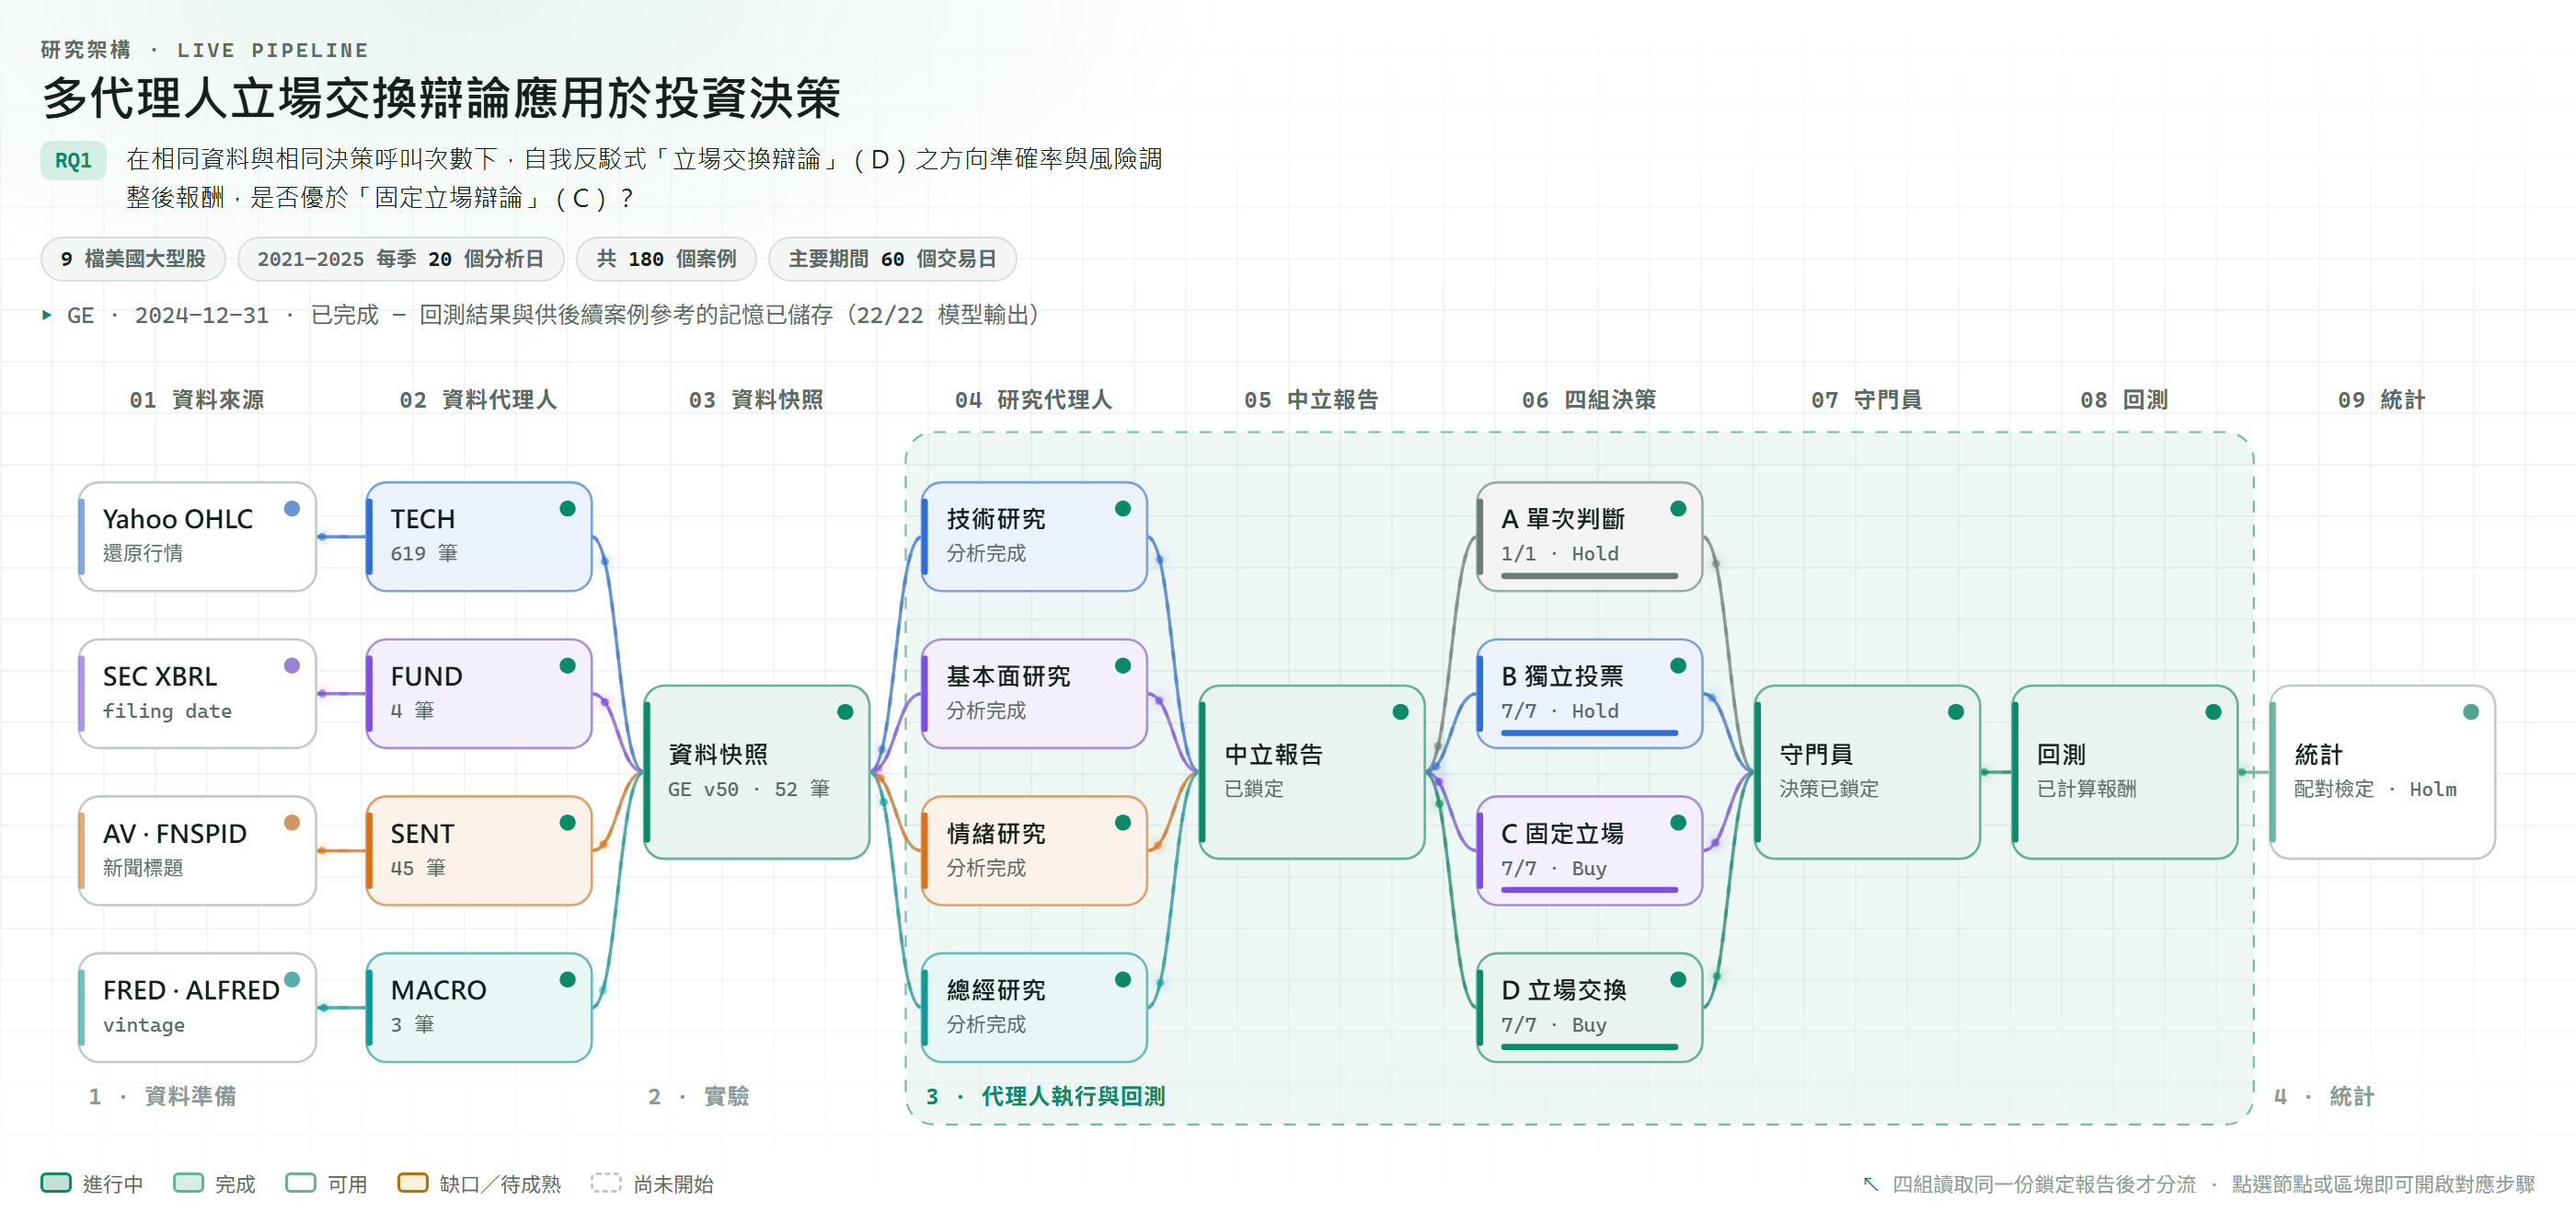
\includegraphics[width=\textwidth]{figures/ui-pipeline.png}}{\fbox{\parbox{0.9\textwidth}{既有介面圖資：原報告 figures/ui-pipeline.png。此單檔預覽以文字保留圖意：資料來源、資料代理人、快照、四類研究代理人、中立報告、決策分支、守門、回測與統計；原截圖保留於既有報告，非新版功能證據。}}}
\caption{網頁介面之資料流向圖（一個已完成案例）。由左至右為資料來源、資料代理人、資料快照、研究代理人、中立報告、四組決策、守門員、回測與統計。}
\label{fig:ui}
\end{figure}
介面以執行狀態與來源追蹤支援研究檢查，模型指派、論證、裁決及資源紀錄均應可對應到單一案例。

\subsection{實作流程與驗證}

\subsubsection{開發流程}
系統依「資料、研究、決策、回測、統計」之順序逐步開發，每完成一個模組即以合成資料與小樣本測試，再以少量真實案例試跑後才進行正式實驗。開發過程中的主要挑戰與對策如下：

\begin{itemize}
  \item 時間邊界：財報與新聞須以「可取得時間」篩選，避免分析日後的資訊進入輸入；總經資料改用歷史版本以排除事後修正。
  \item 模型輸出不穩定：模型常引用不存在的證據或格式錯誤，以結構化輸出、證據短代稱與自動重試處理；模型也常自行改寫數字，改為要求以證據代稱指稱事實。
  \item 結果可重現：實驗跨越多天執行，系統於事前登記時鎖定程式與模型版本，每一步推理前後核對模型權重，版本不符即拒絕執行。
  \item 長時間執行：網路中斷時自動暫停並於恢復後續跑，已完成之步驟不重新產生，確保 180 個案例在一致條件下完成。
\end{itemize}
\subsubsection{Audit Trail 與版本核對}
為使每個決策可回溯，模型輸出寫入前皆經驗證，且每次呼叫皆留下稽核紀錄：

\begin{itemize}
  \item 提示詞中之證據以短代稱（E1、E2、$\ldots$）呈現，回答後由程式對映回真實識別碼，避免模型抄寫長識別碼出錯，同時不使識別碼中之申報編號洩漏公司身分。
  \item 引用之證據必須存在；引用不存在之證據或格式錯誤時，以明確訊息要求重試，最多三次。
  \item 數字檢查：新版要求代理人以證據代稱指稱事實、不重述數字；敘述中仍出現之數字若無任何證據數值支持（期間名稱、日期、來源值之四捨五入或截位不計），僅記錄並依組別報告比例，不重試、不修改文字。
  \item 凍結與身分核對：每一步推理前後皆核對模型權重之 digest，無法取得時暫停並可續跑，確認不同時則該案永久作廢；程式原始碼之雜湊納入協議雜湊，改動即拒絕續跑。連線故障連續發生時暫停派發新案例，並於停滯過久時自動關閉 GPU 主機。
  \item 每個案例可匯出完整紀錄：協議設定、中立報告、證據登錄、執行軌跡、記憶、決策、逐案例回測與彙總指標，以及辯論逐字稿。
\end{itemize}
\subsection{Implementation Challenges}

\subsubsection{異質格式與 context handling}
不同模型的structured output、tokenizer與context能力不同，轉接器不能加入額外金融訊息或默默截去某方反證。需統一輸出契約、保存raw response與截斷紀錄，約束輸入長度並記錄失敗。

\subsubsection{資源公平與 domain output normalization}
相同calls不等於相同tokens、成本或latency；平行四域還有wall-clock與累計推理時間之差。Views長度、缺失值、證據與反證欄位標準化會影響上層裁決，schema與prompt必須先鎖定，不能依事後績效調權重。

\subsubsection{模型能力混淆}
模型路由不等於異質性效果識別；能力組成、Judge文風偏好與不同訓練記憶風險仍可能影響比較，須以模型條件、輸入控制與結果範圍限定解讀。

\section{結果與討論}
\subsection{既有協議的機制比較}
本節呈現qwen3:32b、季度協議v3-1002.3的既有回溯比較，以及同批Gemini探索性分析。其模型、流程與資料身分限定了結果的適用範圍；本節不作為異質模型辯論或領域專業化架構的績效證據。


\subsubsection{舊 qwen 績效與檢定}
180 個事前登記案例全數完成，無排除案例。表~\ref{tab:main} 為四組之績效，表~\ref{tab:tests} 為配對檢定。

\begin{table}[H]
\centering\small
\caption{四組績效（180 案，60 個交易日，扣除交易成本）}
\label{tab:main}
\begin{tabular}{@{}lccccc@{}}
\toprule
組別 & 出手率 & 條件準確率 & 累積報酬 & 最大回撤 & 年化 Sharpe \\
\midrule
\grp{A}\ 單次判斷 & 78.3\% & 56.0\% & 1.85\% & $-1.81\%$ & 0.44 \\
\grp{B}\ 獨立投票 & 79.4\% & 55.9\% & 1.95\% & $-1.83\%$ & 0.46 \\
\grp{C}\ 固定立場辯論 & 100\% & 58.3\% & 2.51\% & $-1.47\%$ & 0.59 \\
\grp{D}\ 立場交換辯論 & 100\% & 55.0\% & 2.11\% & $-2.01\%$ & 0.54 \\
\midrule
買進持有（同案同期間） & -- & -- & 5.60\% & $-1.59\%$ & 1.01 \\
\bottomrule
\end{tabular}
\par\smallskip
\raggedright\footnotesize 決策為守門員之前之候選決策。出手率為買進或賣出（非持有）之比例；方向準確率以有出手之案例計算。組合將每個「股票×分析日」案例視為一個固定權重（1/180）之部位，僅於該案 60 日持有期間依決策做多或放空，其餘時間與持有之案例以零報酬現金計，故不同案例之持有期可能重疊。買進持有基準採相同配置，於每案相同期間做多該股票，並非九檔股票全期間持續持有。
\end{table}

\begin{table}[H]
\centering\small
\caption{立場交換組（\grp{D}）之配對檢定（60 個交易日）}
\label{tab:tests}
\begin{tabular}{@{}lcccccc@{}}
\toprule
比較 & 配對案例 & 方向不同 & 準確率差 & McNemar $p$ & Sharpe 差 & Ledoit--Wolf $p$ \\
\midrule
\grp{D} 對 \grp{C}（主要） & 180 & 16 & $-3.3$ & 0.21 & $-0.05$ & 0.80 \\
\grp{D} 對 \grp{B} & 143 & 9 & $+0.7$ & 1.00 & $+0.08$ & 0.79 \\
\grp{D} 對 \grp{A} & 141 & 8 & $+1.4$ & 0.73 & $+0.10$ & 0.72 \\
\bottomrule
\end{tabular}
\par\smallskip
\raggedright\footnotesize 準確率差單位為百分點。主要比較經 Holm 校正後之 $p$ 值為 0.42（準確率）與 0.80（Sharpe）。與 \grp{A}、\grp{B} 之比較以兩組皆出手之案例計算。
\end{table}

主要比較中，\grp{D} 之方向準確率與 Sharpe 比率皆略低於 \grp{C}，但差異不顯著。以日期為群聚之準確率差 95\% 信賴區間為 $[-7.2, +0.6]$ 個百分點，Sharpe 差區間為 $[-0.47,+0.36]$；30 與 90 日、不計成本、守門員後決策、排除 37 個新聞來源／覆蓋診斷案例等敏感性分析，皆未提供 \grp{D} 優於 \grp{C} 之顯著證據，但部分點估計方向不同（例如 30 日之 Sharpe 差為 $+0.04$）。四組之 Sharpe 點估計均低於相同配置之買進持有參照（未作對基準之優越性檢定）。

\paragraph{檢定力與等效界線。} 未事前訂定等效／非劣性界值，故不能由未顯著宣稱兩組相同或非劣。若固定觀察到的 16 個不一致案例、暫假設案例獨立，以單一準確率端點之雙尾 $\alpha=0.05$ 精確檢定估算，80\% 檢定力所需之期望差約為 6.3 百分點；此條件式 MDE 未納入日期依賴及 Holm／Sharpe 聯合門檻，也不是事前檢定力規劃。

\paragraph{決策分布。} 180 案中有 129 案（72\%）四組決策完全相同，\grp{C} 與 \grp{D} 僅 16 案方向不同。以候選決策計，四組皆以買進為主（\grp{A} 買進 108、持有 39、賣出 33 案；\grp{B} 109、37、34 案；\grp{C} 買進 145、賣出 35 案；\grp{D} 買進 137、賣出 43 案），\grp{D} 之賣出多於 \grp{C}。守門員僅因 INTC 2024-09-30 波動度過高，將四組之賣出降為持有。\grp{A} 與 \grp{B} 之決策幾乎相同，顯示七次投票之多數決大多與單次判斷一致。
\subsubsection{正反分歧案例與未支持解釋}

以下原case分析在結果已知後選取，只供描述，不識別因果機制。原文「研究問題」與「事前標準」均指舊protocol；少數case不代表全16案模式。
\paragraph{與研究目標比較。} 研究問題為「自我反駁式立場交換是否優於固定立場辯論」。依事前指定之判定標準，兩個主要指標皆未顯著為正，因此不支持立場交換優於一般辯論。辯論兩組之 Sharpe 雖高於 \grp{A}、\grp{B}，但兩組必須出手，在以上漲為主之期間較少持有，此差異不能歸因於辯論本身。

\paragraph{案例一：INTC 2024-03-31（\grp{D} 正確）。} 研究報告顯示新聞情緒偏正面、近 20 日報酬為正，但營收、淨利與營業現金流皆較去年同期大幅衰退。表~\ref{tab:case} 為兩組之辯論與裁決摘要（代理人原文為英文，此為摘譯）。

\begin{table}[H]
\centering\small
\caption{案例一：INTC 2024-03-31 之辯論與裁決（60 日實際報酬 $-30.5\%$）}
\label{tab:case}
\begin{tabularx}{\textwidth}{@{}l l Y@{}}
\toprule
組別／輪次 & 立場與預測 & 論點摘要 \\
\midrule
\grp{C} 第 1--3 輪 & 看多 $+8\%$；看空 $-12\%$ & 看多方三輪幾乎重複「情緒正面與短期動能支持看多」；看空方亦重複財報衰退，雙方未回應對方核心證據 \\
\grp{C} 裁決 & 買進，$+5\%$ & 採納看多方之短期動能論點 \\
\midrule
\grp{D} 第 1 輪 & 看多 $+8\%$；看空 $-10\%$ & 與 \grp{C} 相同之兩種論點 \\
\grp{D} 第 2 輪 & 原看多者改看空，$-7\%$ & 引用並反駁自己的原主張：正面情緒與短期報酬「被營收、淨利與現金流之大幅衰退所抵銷」 \\
\grp{D} 裁決 & 賣出，$-7\%$ & 基本面惡化之重要性高於短期情緒 \\
\bottomrule
\end{tabularx}
\end{table}

此案中可觀察到交換輪強調原先被輕描淡寫的基本面衰退，且最終裁決轉為賣出；60 日後股價下跌 30.5\%，\grp{C} 是四組中唯一判斷錯誤者。

\paragraph{案例二：AAPL 2023-03-31（\grp{D} 錯誤）。} 此案技術面強勁（近 20 日上漲 11.3\%），但營收與淨利年減；\grp{C} 採納技術動能判斷買進，\grp{D} 之交換輪則再次強調基本面衰退，裁決者判斷賣出。60 日後股價上漲 15.3\%，\grp{D} 錯誤。

\paragraph{整體模式。} 在 16 個方向不同的案例中，\grp{D} 有 12 案判斷賣出；就全部 16 案而言，D 正確 5 案、C 正確 11 案。兩個案例中皆可觀察到交換輪強調反面證據（多為基本面衰退），且 \grp{D} 之最終決策較常轉為看空，此模式與自我反駁之設計目的相符；但少數案例不足以確認其因果機制。可能的解釋是：本研究期間以上漲為主，「基本面疲弱而股價續漲」之情形較多，較常看空反而不利。兩組的部分文字與決策不同，但未支持 D 較佳；不能將差異全歸因於交換立場。此結論亦與「辯論效果常被高估」之文獻一致 \citep{smit2023mad,zhang2025stop}。
\subsection{Exploratory Cross-model Analysis 與前導診斷}

\subsubsection{Gemini homogeneous 比較}

整套系統改用 Gemini 仍然是 homogeneous-model setting，不等於新版 RQ2 所研究的 heterogeneous debate。以下從較詳盡原稿保留同批探索性結果及未支持假說；舊文的跨模型RQ2不再列正式Research Question。


以下分析皆於主要結果揭曉後進行，未列入事前登記，依 \citet{wagenmakers2012agenda} 與 \citet{nosek2018prereg} 之區分屬探索性分析，僅用於產生後續研究之假說，不作為確認性證據。

\paragraph{跨模型比較。} 原分析以 Gemini 3 Flash 依相同案例集合、流程與匿名化設定重跑四組（表~\ref{tab:flash}）。結果與 qwen3:32b 一致：\grp{D} 之準確率仍略低於 \grp{C}，\grp{C}、\grp{D} 方向不同之案例僅 9 案（\grp{D} 單獨正確 3 案、\grp{C} 單獨正確 6 案，McNemar $p=0.51$）。此為相同標的、日期與來源資訊上的模型替換比較，不是獨立資料複製。現有匯出紀錄不足以證明兩模型的完整呼叫設定與逐案研究報告身分一致，因此不能宣稱兩模型逐位元讀取相同報告，或將模型替換解讀為純能力改變。兩模型之決策高度相似，\grp{C}、\grp{D} 分別有 165 與 162 案方向相同。

\begin{table}[H]
\centering\small
\caption{跨模型比較：方向準確率（60 日、候選決策、有出手之案例）}
\label{tab:flash}
\begin{tabular}{@{}lcc@{}}
\toprule
組別 & qwen3:32b & Gemini 3 Flash \\
\midrule
\grp{A} 單次判斷 & 56.0\% & 57.6\% \\
\grp{B} 獨立投票 & 55.9\% & 56.7\% \\
\grp{C} 固定立場辯論 & 58.3\% & 57.8\% \\
\grp{D} 立場交換辯論 & 55.0\% & 56.1\% \\
\midrule
一律看多（全 180 案；僅與 C／D 同基底） & \multicolumn{2}{c}{62.2\%} \\
\bottomrule
\end{tabular}
\par\smallskip
\raggedright\footnotesize 兩模型均報告 180 案。qwen 的 A、B 有出手案例為 141、143 案（覆蓋率 78.3\%、79.4\%），C、D 為 180 案。現有Gemini彙總未提供可核對的A/B出手數及覆蓋率；C、D 依強制下注規則為 180 案。A、B 的條件準確率不能直接與全樣本 62.2\% 比較；本文不將其出手子集與全樣本看多基準直接比較。
\end{table}

\paragraph{與一律看多之比較。} 180 案中 112 案於 60 日內上漲（62.2\%）、68 案下跌（37.8\%）。只有覆蓋全部案例的 \grp{C}、\grp{D} 可直接與此事後方向參照比較；兩模型的這兩組準確率點估計均較低。對 qwen，表~\ref{tab:confusion} 由既有決策總數與正確數重建完整分布，不作為新的逐案驗證。賣出精確率分別為 40.0\%（14/35）與 34.9\%（15/43），相對全樣本下跌率 37.8\% 一高一低；下跌召回率為 20.6\% 與 22.1\%。因此可描述其下跌召回偏低，不能概括為完全沒有辨識力。

\begin{table}[H]
\centering\small
\caption{qwen3:32b 的方向混淆分布（60 日，候選決策）}
\label{tab:confusion}
\begin{tabular}{@{}llrrr@{}}
\toprule
組別 & 預測方向 & 實際上漲 & 實際下跌 & 合計 \\
\midrule
\grp{C} & 買進 & 91 & 54 & 145 \\
         & 賣出 & 21 & 14 & 35 \\
\grp{D} & 買進 & 84 & 53 & 137 \\
         & 賣出 & 28 & 15 & 43 \\
\bottomrule
\end{tabular}
\par\smallskip
\raggedright\footnotesize 每組總數 180；正確數 C=105、D=99。由既有彙總數代數重建，不視為額外逐案驗證。A／B 的持有分布與 Gemini 的完整分布不由四捨五入準確率反推。
\end{table}

\paragraph{本資料未支持的解釋。} 本研究原推測 \grp{D} 較常看空，因而在多頭期吃虧、在空頭期應較佳。將 20 個分析日依九檔平均 60 日報酬分為 6 個空頭季與 14 個多頭季後，\grp{D} 在空頭季之準確率亦未高於 \grp{C}（qwen 24.1\% 對 25.9\%；Flash 25.9\% 對 27.8\%），各模型僅相差一案，且季別為事後分類；此資料未能支持上述推測，但不能宣稱已否證。

\paragraph{對舊跨模型探索問題之回答。} 兩模型之 \grp{D}$-$\grp{C} 準確率差均為負，符合舊跨模型探索問題對「差異方向一致」的描述性定義；未檢定模型與機制交互作用、等效性或跨模型 Sharpe 的聯合判準。因使用同批樣本、分析屬探索性且模型紀錄完整度有限，不能宣稱已確認跨模型穩健性。

\paragraph{後續假說。} 本研究在兩個模型的既有準確率結果中均未觀察到 \grp{D} 改善。輸入資訊之預測力不足是可能解釋之一，但市場噪音與效率、提示設計、模型限制、樣本數及生成變異也可能造成此結果，本文未以實驗區分。後續可在新期間或新標的，先登記資訊集擴充與消融方案，再檢驗跨標的訊號是否有增量價值 \citep{nosek2018prereg}；不可在同一批產生假說的資料上將探索結果改稱確認性證據。
\subsubsection{舊協議記憶與匿名辨識探針}
\label{sec:memorydiagnostic}

專案已保存 2026 年 9 月 28 日 qwen3:32b 的前導探針，無資料回想測試使用 63 題、60 日期間、溫度 0、種子 905；2022、2023、2024 年各 9 題的方向正確率為 33.3\%、33.3\%、55.6\%，2025 年 36 題為 72.2\%，皆未高於各組多數方向基準（66.7\%、66.7\%、55.6\%、72.2\%）。這只能說明此問法未觀察到超越基準的回想表現，不證明沒有記憶。

另以 2023-06-30、2024-06-30 各九檔的匿名證據前 6,000 字元詢問公司身分，qwen 辨識 6/18（33.3\%）；產品名稱與財報規模仍提供線索。此為開放式公司回答，不是九選一測試，故不直接採 1/9 作統計虛無基準。兩項探針使用舊協議 39f71a9c，未完整保留可比對的模型權重與新版研究報告身分；不能當作 v3-1002.3 全部 180 案之辨識率。專案另有 Gemini 2.5 Flash 等舊模型探針，也不能替代本批 Gemini 3 Flash 的汙染檢驗。


\subsection{研究限制}

\subsubsection{資料有效性}
九檔為資料可取得性導向的目的性樣本，未納入退市公司，存在存活與事後選樣風險。財報filing date、macro historical vintage與新聞timestamp控制資料可得時間，但不排除模型訓練記憶；匿名化仍保留數值、日期及產品線索。行情採下載時的調整版本，也存在事後修訂風險。新聞來源與密度隨年份及個股改變；37案排除分析僅是來源／覆蓋診斷，不能外推為統一密度門檻。

\subsubsection{實驗有效性}
D同時包含立場交換、隔離對手、強制引用與驗證重試，估計量是整套流程差，而非單一立場交換效果。相同名目呼叫數不代表重試、tokens或compute相同。既有C/D須下注且可用成熟記憶，A/B可持有且無記憶，補充比較混合多項差異。各案採單次生成，觀察到的C/D分歧同時可能含生成噪音。同批資料已用於前導及規則調整，規則鎖定不能恢復未見樣本的確認性。

異質模型與能力組成、訓練記憶差異難以完全分離；同temperature或seed不代表相同生成機制。領域切分可能遺失跨域互動，上層整合也受輸入順序、長度與文風影響。模型輸出多樣性及論述豐富程度不能直接作為績效改善證據。

\subsubsection{統計有效性}
180案共享20個日期與重疊持有期，主要C/D比較只有16個不一致案例。日期群聚區間用於依賴性敏感度檢查，不當作等效或非劣證據；條件式MDE也不是事前研究檢定力。由於未事前登記等效界值，不以不顯著結果宣稱兩流程相同。Sharpe以對齊日序列計算，其觀測數T與案例數180、日期群聚數20不可互換。

\subsubsection{外部有效性與可重現性}
結果限定九檔美國大型股、2021--2025年與指定模型／協議，不能推廣至全部市場。Gemini比較共用同批案例，不是獨立複製；現有匯出不能支持兩模型逐位元讀取相同研究報告的主張。FinBERT revision、完整Gemini呼叫設定與行情調整版本的紀錄完整度限制精確重現。既有小樣本匿名探針的辨識率也不代表全部180案。


\section{結論與建議}



\subsection{應用與價值}

\subsubsection{可追溯決策輔助}
在應用上，本系統可作為投資研究之輔助工具：將資料整理、正反論證、裁決理由與回測結果完整保留，使用者能追溯每一個建議的依據，而非只得到一個買賣訊號。在方法上，本研究示範如何以決策呼叫次數對齊、事前登記、匿名化與版本鎖定評估語言模型代理人，避免「呼叫次數較多」或「事後挑選結果」造成的誤判；此評估框架亦可用於其他多代理人設計之比較。
\subsubsection{Multi-Agent System Design}

研究價值也在於系統設計的可辨識比較：不同代理人名稱不足以證明有用差異；是否需要heterogeneous models、複雜資訊是否適合specialists、以及domain decomposition的效益都應以受控結果與成本評估回答。若未觀察改善，仍可提供架構適用邊界與可重現評估經驗，不能把負面結果改成分工必然有用。

\subsection{未來展望}

\subsubsection{Temporal-scale robustness}

原月度／20日設計移為Temporal-scale robustness。較短尺度是否減輕一次整合資訊的負担需另做研究，不等同本次domain分工；月度／20日比較採獨立設計，不併入本研究180個季度案例。

\subsubsection{模型、路由、消融及獨立樣本外}

後續可考慮更多模型、heterogeneous Judge、adaptive routing、dynamic debate、domain weighting、compute efficiency與不同辯論輪數。保留原只讀自身但不換立場的消融、空頭及高波動檢查、同案多種子C/C'重跑與完整汙染探針；參數與權重學習須另有開發／驗證資料，最後採新期間或新標的獨立樣本外評估，不在同批產生假說的資料上改稱確認性證據。

\clearpage
\setcounter{section}{7}
\renewcommand{\refname}{七、參考文獻}
\addcontentsline{toc}{section}{七、參考文獻}
\begin{thebibliography}{99}

\bibitem[\protect\citeauthoryear{Araci}{Araci}{2019}]{araci2019finbert}
Araci, D. (2019).
\newblock FinBERT: Financial sentiment analysis with pre-trained language
  models.
\newblock arXiv preprint arXiv:1908.10063.
\newblock \url{https://doi.org/10.48550/arXiv.1908.10063}.

\bibitem[Chen et al., 2023]{chen2023agentverse}
Chen, W., Su, Y., Zuo, J., Yang, C., Yuan, C., Chan, C.-M., Yu, H., Lu, Y., Hung, Y.-H., Qian, C., Qin, Y., Cong, X., Xie, R., Liu, Z., Sun, M., and Zhou, J. (2023).
\newblock AgentVerse: Facilitating Multi-Agent Collaboration and Exploring Emergent Behaviors.
\newblock arXiv preprint arXiv:2308.10848v3.
\newblock \url{https://arxiv.org/abs/2308.10848v3}.

\bibitem[\protect\citeauthoryear{Chen, Luo, Wu, and Mou}{Chen
  et~al.}{2026}]{chen2026mpt}
Chen, Y., G.~Luo, Z.~Wu, and L.~Mou (2026).
\newblock Multi-persona thinking for bias mitigation in large language models.
\newblock In {\em Findings of the Association for Computational Linguistics:
  ACL 2026}, pp.\  27895--27909.

\bibitem[\protect\citeauthoryear{Chowdhury, Beg, Khan, Raiyan, Hasan, and
  Mahmud}{Chowdhury et~al.}{2026}]{chowdhury2026proclaim}
Chowdhury, M.~N., N.~J. Beg, U.~H. Khan, S.~R. Raiyan, M.~K. Hasan, and
  H.~Mahmud (2026).
\newblock Courtroom-style multi-agent debate with progressive {RAG} and
  role-switching for controversial claim verification.
\newblock arXiv preprint arXiv:2603.28488v1.
\newblock \url{https://doi.org/10.48550/arXiv.2603.28488}.

\bibitem[\protect\citeauthoryear{Corwin and Schultz}{Corwin and
  Schultz}{2012}]{corwin2012spread}
Corwin, S.~A. and P.~Schultz (2012).
\newblock A simple way to estimate bid-ask spreads from daily high and low
  prices.
\newblock {\em The Journal of Finance\/}~{\em 67\/}(2), 719--760.

\bibitem[\protect\citeauthoryear{Dong, Fan, and Peng}{Dong
  et~al.}{2024}]{dong2024fnspid}
Dong, Z., X.~Fan, and Z.~Peng (2024).
\newblock FNSPID: A comprehensive financial news dataset in time series.
\newblock arXiv preprint arXiv:2402.06698.
\newblock \url{https://doi.org/10.48550/arXiv.2402.06698}.

\bibitem[\protect\citeauthoryear{Du, Li, Torralba, Tenenbaum, and Mordatch}{Du
  et~al.}{2023}]{du2023debate}
Du, Y., S.~Li, A.~Torralba, J.~B. Tenenbaum, and I.~Mordatch (2023).
\newblock Improving factuality and reasoning in language models through
  multiagent debate.
\newblock arXiv preprint arXiv:2305.14325.
\newblock \url{https://doi.org/10.48550/arXiv.2305.14325}.

\bibitem[\protect\citeauthoryear{Glasserman and Lin}{Glasserman and
  Lin}{2023}]{glasserman2023lookahead}
Glasserman, P. and C.~Lin (2023).
\newblock Assessing look-ahead bias in stock return predictions generated by
  GPT sentiment analysis.
\newblock arXiv preprint arXiv:2309.17322.
\newblock \url{https://doi.org/10.48550/arXiv.2309.17322}.

\bibitem[\protect\citeauthoryear{Holm}{Holm}{1979}]{holm1979}
Holm, S. (1979).
\newblock A simple sequentially rejective multiple test procedure.
\newblock {\em Scandinavian Journal of Statistics\/}~{\em 6\/}(2), 65--70.

\bibitem[\protect\citeauthoryear{Huang, Chen, Mishra, Zheng, Yu, Song, and
  Zhou}{Huang et~al.}{2024}]{huang2024selfcorrect}
Huang, J., X.~Chen, S.~Mishra, H.~S. Zheng, A.~W. Yu, X.~Song, and D.~Zhou
  (2024).
\newblock Large language models cannot self-correct reasoning yet.
\newblock In {\em International Conference on Learning Representations}.

\bibitem[\protect\citeauthoryear{Jobson and Korkie}{Jobson and
  Korkie}{1981}]{jobson1981sharpe}
Jobson, J.~D. and B.~M. Korkie (1981).
\newblock Performance hypothesis testing with the Sharpe and Treynor measures.
\newblock {\em The Journal of Finance\/}~{\em 36\/}(4), 889--908.

\bibitem[\protect\citeauthoryear{Kong, Lee, Hwang, Lopez-Lira, Levy, Mehta,
  Wen, Choi, Lee, and Zohren}{Kong et~al.}{2026}]{kong2026bias}
Kong, Y., H.~Lee, Y.~Hwang, A.~Lopez-Lira, B.~Levy, D.~Mehta, Q.~Wen, C.~Choi,
  Y.~Lee, and S.~Zohren (2026).
\newblock Evaluating {LLMs} in finance requires explicit bias consideration.
\newblock arXiv preprint arXiv:2602.14233v1.
\newblock \url{https://doi.org/10.48550/arXiv.2602.14233}.

\bibitem[\protect\citeauthoryear{Ledoit and Wolf}{Ledoit and
  Wolf}{2008}]{ledoit2008sharpe}
Ledoit, O. and M.~Wolf (2008).
\newblock Robust performance hypothesis testing with the Sharpe ratio.
\newblock {\em Journal of Empirical Finance\/}~{\em 15\/}(5), 850--859.

\bibitem[\protect\citeauthoryear{Liang, He, Jiao, Wang, Wang, Wang, Yang, Tu,
  and Shi}{Liang et~al.}{2023}]{liang2023divergent}
Liang, T., Z.~He, W.~Jiao, X.~Wang, Y.~Wang, R.~Wang, Y.~Yang, Z.~Tu, and
  S.~Shi (2023).
\newblock Encouraging divergent thinking in large language models through
  multi-agent debate.
\newblock arXiv preprint arXiv:2305.19118v1.
\newblock \url{https://doi.org/10.48550/arXiv.2305.19118}.

\bibitem[\protect\citeauthoryear{Liu, Wang, Yang, and Zha}{Liu
  et~al.}{2023}]{liu2023fingpt}
Liu, X.-Y., G.~Wang, H.~Yang, and D.~Zha (2023).
\newblock {FinGPT}: Democratizing internet-scale data for financial large
  language models.
\newblock arXiv preprint arXiv:2307.10485.
\newblock \url{https://doi.org/10.48550/arXiv.2307.10485}.

\bibitem[\protect\citeauthoryear{Liu, Khajavi, Jiang, and Liu}{Liu
  et~al.}{2025}]{liu2025roleswitch}
Liu, Z., S.~Khajavi, G.~Jiang, and X.~Liu (2025).
\newblock Uncertainty-aware role-switching debate: Improving truthfulness in
  large language models.
\newblock OpenReview, \url{https://openreview.net/forum?id=heYWeCpOlS}.

\bibitem[\protect\citeauthoryear{Lopez-Lira and Tang}{Lopez-Lira and
  Tang}{2023}]{lopezlira2023chatgpt}
Lopez-Lira, A. and Y.~Tang (2023).
\newblock Can {ChatGPT} forecast stock price movements? return predictability
  and large language models.
\newblock arXiv preprint arXiv:2304.07619.
\newblock \url{https://doi.org/10.48550/arXiv.2304.07619}.

\bibitem[\protect\citeauthoryear{Lord, Lepper, and Preston}{Lord
  et~al.}{1984}]{lord1984opposite}
Lord, C.~G., M.~R. Lepper, and E.~Preston (1984).
\newblock Considering the opposite: A corrective strategy for social judgment.
\newblock {\em Journal of Personality and Social Psychology\/}~{\em 47\/}(6),
  1231--1243.

\bibitem[\protect\citeauthoryear{McNemar}{McNemar}{1947}]{mcnemar1947}
McNemar, Q. (1947).
\newblock Note on the sampling error of the difference between correlated
  proportions or percentages.
\newblock {\em Psychometrika\/}~{\em 12\/}(2), 153--157.

\bibitem[\protect\citeauthoryear{Nosek, Ebersole, DeHaven, and Mellor}{Nosek
  et~al.}{2018}]{nosek2018prereg}
Nosek, B.~A., C.~R. Ebersole, A.~C. DeHaven, and D.~T. Mellor (2018).
\newblock The preregistration revolution.
\newblock {\em Proceedings of the National Academy of Sciences\/}~{\em
  115\/}(11), 2600--2606.

\bibitem[\protect\citeauthoryear{Smit, Duckworth, Grinsztajn, Barrett, and
  Pretorius}{Smit et~al.}{2023}]{smit2023mad}
Smit, A., P.~Duckworth, N.~Grinsztajn, T.~D. Barrett, and A.~Pretorius (2023).
\newblock Should we be going {MAD}? a look at multi-agent debate strategies for
  {LLMs}.
\newblock arXiv preprint arXiv:2311.17371.
\newblock \url{https://doi.org/10.48550/arXiv.2311.17371}.

\bibitem[\protect\citeauthoryear{Wagenmakers, Wetzels, Borsboom, van~der Maas,
  and Kievit}{Wagenmakers et~al.}{2012}]{wagenmakers2012agenda}
Wagenmakers, E.-J., R.~Wetzels, D.~Borsboom, H.~L.~J. van~der Maas, and R.~A.
  Kievit (2012).
\newblock An agenda for purely confirmatory research.
\newblock {\em Perspectives on Psychological Science\/}~{\em 7\/}(6), 632--638.

\bibitem[Wang et al., 2024]{wang2024moa}
Wang, J., Wang, J., Athiwaratkun, B., Zhang, C., and Zou, J. (2024).
\newblock Mixture-of-Agents Enhances Large Language Model Capabilities.
\newblock arXiv preprint arXiv:2406.04692v1.
\newblock \url{https://arxiv.org/abs/2406.04692v1}.

\bibitem[\protect\citeauthoryear{Wang, Wei, Schuurmans, Le, Chi, Narang,
  Chowdhery, and Zhou}{Wang et~al.}{2023}]{wang2023selfconsistency}
Wang, X., J.~Wei, D.~Schuurmans, Q.~Le, E.~Chi, S.~Narang, A.~Chowdhery, and
  D.~Zhou (2023).
\newblock Self-consistency improves chain of thought reasoning in language
  models.
\newblock In {\em International Conference on Learning Representations}.

\bibitem[\protect\citeauthoryear{Xiao, Sun, Luo, and Wang}{Xiao
  et~al.}{2024}]{xiao2024tradingagents}
Xiao, Y., E.~Sun, D.~Luo, and W.~Wang (2024).
\newblock TradingAgents: Multi-agents llm financial trading framework.
\newblock arXiv preprint arXiv:2412.20138.
\newblock \url{https://doi.org/10.48550/arXiv.2412.20138}.

\bibitem[Yang et al., 2024]{yang2024finrobot}
Yang, H., Zhang, B., Wang, N., Guo, C., Zhang, X., Lin, L., Wang, J., Zhou, T., Guan, M., Zhang, R., and Wang, C. D. (2024).
\newblock FinRobot: An Open-Source AI Agent Platform for Financial Applications using Large Language Models.
\newblock arXiv preprint arXiv:2405.14767v2.
\newblock \url{https://arxiv.org/abs/2405.14767v2}.

\bibitem[\protect\citeauthoryear{Zhang, Liu, Zhang, Jin, Li, Wang, Hua, Shu,
  Zhu, Jin, Li, Du, and Zhang}{Zhang et~al.}{2024}]{zhang2024stockagent}
Zhang, C., X.~Liu, Z.~Zhang, M.~Jin, L.~Li, Z.~Wang, W.~Hua, D.~Shu, S.~Zhu,
  X.~Jin, S.~Li, M.~Du, and Y.~Zhang (2024).
\newblock When {AI} meets finance ({StockAgent}): Large language model-based
  stock trading in simulated real-world environments.
\newblock arXiv preprint arXiv:2407.18957.
\newblock \url{https://doi.org/10.48550/arXiv.2407.18957}.

\bibitem[\protect\citeauthoryear{Zhang, Cui, Chen, Wang, Zhang, Wang, Wu, and
  Hu}{Zhang et~al.}{2025}]{zhang2025stop}
Zhang, H., Z.~Cui, J.~Chen, X.~Wang, Q.~Zhang, Z.~Wang, D.~Wu, and S.~Hu
  (2025).
\newblock Stop overvaluing multi-agent debate -- we must rethink evaluation and
  embrace model heterogeneity.
\newblock arXiv preprint arXiv:2502.08788.
\newblock \url{https://doi.org/10.48550/arXiv.2502.08788}.

\bibitem[Zheng et al., 2023]{zheng2023judge}
Zheng, L., Chiang, W.-L., Sheng, Y., Zhuang, S., Wu, Z., Zhuang, Y., Lin, Z., Li, Z., Li, D., Xing, E. P., Zhang, H., Gonzalez, J. E., and Stoica, I. (2023).
\newblock Judging LLM-as-a-Judge with MT-Bench and Chatbot Arena.
\newblock arXiv preprint arXiv:2306.05685v4.
\newblock \url{https://arxiv.org/abs/2306.05685v4}.

\end{thebibliography}

\vspace{0.3cm}
\noindent\small 本文僅供學術研究與教學使用，不構成任何投資建議。
\end{CJK}
\end{document}
